\newpage
\section{Arquitectura física del sistema}
En la figura \ref{fig:DisenoArquiFisica} se muestra la arquitectura física del sistema, la cual abarca el diseño de la aplicación móvil así como el sistema embebido encargado de realizar las mediciones.\\

El diagrama está compuesto por dos módulos, los cuales se describen a continuación:
\begin{enumerate}
	\item Aplicación Móvil: se refiere a la aplicación móvil que proporcionará un punto de acceso al usuario para la consulta de las mediciones realizadas por los sensores y procesadas por el microcontrolador en el sistema embebido. 
	\item Sistema Embebido: abarca todos los componentes que integran el sistema embebido como tal. En este módulo se realizan los cálculos necesarios para la obtención de la frecuencia cardíaca y la temperatura corporal y el envío de estas mediciones al usuario mediante mensajes de texto.
\end{enumerate}

\begin{figure}[htbp!]
	\centering
	\fbox{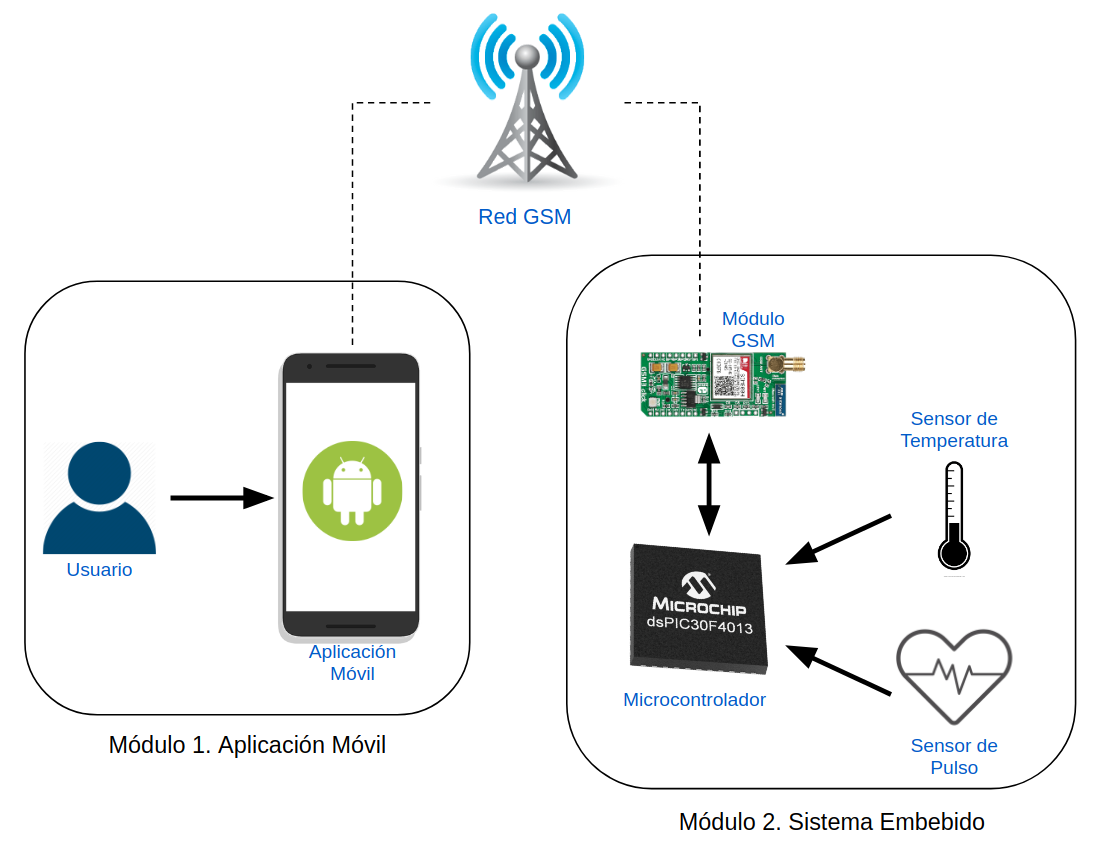
\includegraphics[width=0.9\textwidth]{DisenoEstructura/imagenes/arquifisica.png}}
	\caption{Arquitectura física del sistema}
	\label{fig:DisenoArquiFisica}
\end{figure}
\clearpage

\section{Arquitectura lógica del sistema}
Una vez definidos los componentes que serán utilizados para constituir el sistema embebido, se definió la arquitectura lógica del sistema mostrada en la figura \ref{fig:DisenoArquiLogica}, especificando la forma en que se realizará la comunicación entre componentes.\\

La arquitectura planteada se divide en tres partes, las cuales definen la forma de comunicación entre el sistema embebido, la red 3G/4G y la aplicación móvil.\\

\begin{figure}[htbp!]
	\centering
	\fbox{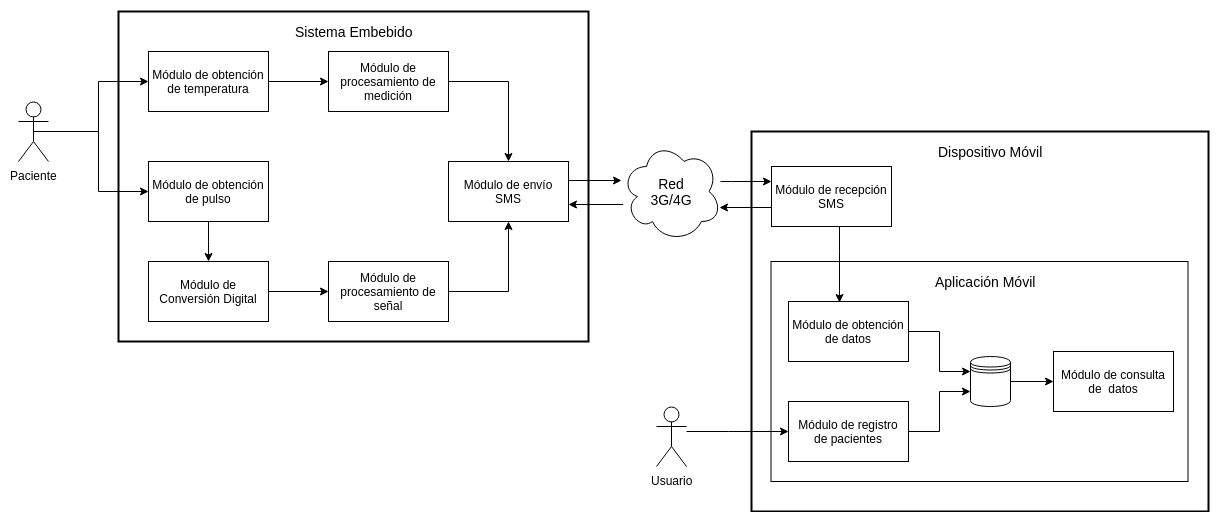
\includegraphics[width=\textwidth]{DisenoEstructura/imagenes/arquitectura.png}}
	\caption{Arquitectura lógica del sistema}
	\label{fig:DisenoArquiLogica}
\end{figure}

El sistema embebido se encarga de obtener la señal de pulso cardíaco del paciente mediante el sensor de pulso a través de una entrada analógica, este señal es enviada al módulo de conversión digital en donde es digitalizada para posteriormente enviarla al módulo de procesamiento digital, en donde será procesada para obtener la frecuencia cardíaca. Para la obtención y cálculo de la temperatura, se tiene el módulo de obtención de temperatura y de procesamiento de medición. \\

Estos valores se envían al módulo de comunicación, con el que se realizará el envío de mensajes de texto mediante la red 3G/4G hacia el dispositivo móvil. \\

El usuario recibe el mensaje en su dispositivo móvil mediante el módulo de recepción SMS y la aplicación móvil obtendrá los datos de dicho mensaje mediante el módulo de obtención de datos. El usuario podrá registrar la información del paciente mediante el módulo de registro de pacientes. Los dos módulos anteriores proporcionarán la información que será almacenada en una base de datos de la cual el módulo de consulta de datos obtendrá la información para mostrarla al usuario.